\documentclass{standalone}
\usepackage{tikz}
\usepackage{ctex,siunitx}
\setCJKmainfont{Noto Serif CJK SC}
\usepackage{tkz-euclide}
\usepackage{amsmath}
\usetikzlibrary{patterns, calc}
\usetikzlibrary {decorations.pathmorphing,decorations.pathreplacing,decorations.shapes,}
\begin{document}
\small
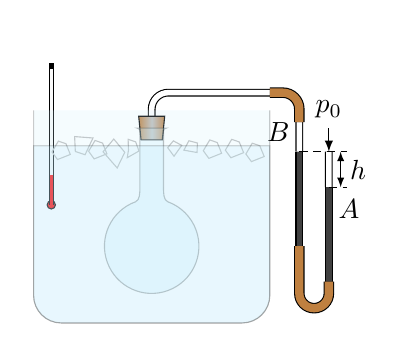
\begin{tikzpicture}[>=latex,scale=0.75]
  \useasboundingbox(-2.1,-1.4)rectangle(3.65,3.7);
  \draw[double,double distance=2pt,rounded corners=6pt](0,2.0)--(0,2.6)--(2.5,2.6)--(2.5,1.6)(3.0,1.0)--(3.0,1.6);
  \draw[double=brown,double distance=3pt,rounded corners=6pt](2.0,2.6)--(2.5,2.6)--(2.5,2.1);
  \draw[double=darkgray,double distance=2pt](2.5,1.6)node[above left]{$B$}--(2.5,0)(3.0,1.0)--(3.0,-0.6);
  \node at (3.0,0.3) [above right]{$A$};
  \draw[very thin,<->](3.2,1.6)--(3.2,1.0)node[right,midway]{$h$};
  \draw[very thin, densely dashed] (2.5,1.6)--(3.3,1.6)(3.0,1)--(3.3,1);
  \draw[double=brown,double distance=3pt](2.5,0)--++(0,-0.8)arc(180:360:0.25)--++(0,0.2);
  \draw[left color=brown,right color=brown,middle color=lightgray](-0.18,1.8)--(-0.22,2.2)--(0.22,2.2)--(0.18,1.8)--cycle;
  \draw[fill=cyan!20,opacity=0.3](0,2.0)--(-0.25,2.0)arc(90:0:0.05)--(-0.2,1)..controls(-0.2,0.9)and(-0.2,0.7785)..(110:0.8)arc(110:430:0.8)..controls(0.2,0.7785)and(0.2,0.9)..(0.2,1)--(0.2,1.95)arc(180:90:0.05)--cycle;
  \draw[thin,->](3,2.0)--++(0,-0.4)node[at start,above]{$p_0$};
  \draw[fill=red](-1.7,0.7)circle(2pt);
  \draw[double=red,double distance=1pt](-1.7,0.7)--(-1.7,1.2);
  \draw[double=lightgray!10,double distance=1pt](-1.7,1.2)--(-1.7,3.0);
  \draw[double=black,double distance=1pt](-1.7,3.0)--(-1.7,3.1);
  \draw[lightgray](-1.688,1.596)--(-1.580,1.779)--(-1.452,1.735)--(-1.378,1.553)--(-1.595,1.467)--cycle
  (-1.293,1.604)--(-1.305,1.856)--(-0.994,1.832)--(-1.128,1.549)--cycle
  (-1.068,1.607)--(-0.959,1.790)--(-0.832,1.746)--(-0.758,1.564)--(-0.974,1.478)--cycle
  (-0.823,1.598)--(-0.642,1.814)--(-0.456,1.590)--(-0.584,1.324)--cycle
  (-0.393,1.625)--(-0.399,1.810)--(-0.271,1.766)--(-0.216,1.611)--(-0.414,1.498)--cycle
  ( 0.378,1.523)--( 0.271,1.668)--( 0.367,1.783)--( 0.509,1.707)--cycle
  ( 0.545,1.626)--( 0.630,1.785)--( 0.775,1.747)--( 0.767,1.586)--cycle
  ( 0.874,1.616)--( 0.983,1.799)--( 1.110,1.755)--( 1.184,1.573)--( 0.968,1.487)--cycle
  ( 1.247,1.626)--( 1.355,1.809)--( 1.483,1.765)--( 1.557,1.583)--( 1.341,1.497)--cycle
  ( 1.595,1.561)--( 1.703,1.744)--( 1.831,1.700)--( 1.905,1.518)--( 1.688,1.432)--cycle;
  \draw[fill=cyan!30,opacity=0.2,rounded corners=10pt](-2,1.7)--(-2,-1.3)--(2,-1.3)[sharp corners]--(2,1.7)--cycle;
  \draw[fill=cyan!20,opacity=0.2,rounded corners=10pt](-2,2.3)--(-2,-1.3)--(2,-1.3)--(2,2.3);
\end{tikzpicture}
\end{document}